\section{Apresentação da plataforma desenvolvida}\label{chap:plataforma-final}

\subsection{Organização e entrada espacial}

A exploração de uma região começa pela definição da área e do período. A interface reúne busca, datas, índices e acionamento da análise em torno do mapa, que recebe a demarcação antes do processamento e apresenta a composição temática depois dele. Esse fluxo permite consultar os produtos sem que o usuário tenha de manipular diretamente os arquivos raster.

\capturatcc{cap01_interface}{CAP-01}{Interface inicial, com controles analíticos e mapa de seleção}{}
\capturatcc{cap02_busca}{CAP-02}{Busca geográfica por Passo Fundo e enquadramento do mapa-base}{}

A busca resolve um nome de lugar e aproxima a navegação da região desejada, sem identificar automaticamente limites cadastrais. O mapa-base é distinto da imagem Sentinel-2 utilizada nos cálculos; sua atribuição acompanha a visualização.

A demarcação fornece a geometria das consultas. Área em hectares, perímetro e centroide permitem conferir o recorte espacial; não são estimativa de área cultivada. O salvamento associa nome e polígono, e a restauração permite repetir análises com outra configuração temporal sem redesenhar a região.

\capturatcc{cap03_poligono}{CAP-03}{Polígono demonstrativo e contexto de seleção espacial}{}
\capturatcc{cap04_salvar}{CAP-04}{Associação de nome à geometria em diálogo de salvamento}{}
\capturatcc{cap05_restaurar}{CAP-05}{Localização restaurada para reutilização da geometria}{}

O armazenamento web está vinculado à sessão. A transferência GeoJSON oferece continuidade por arquivo: exporta localizações e permite importar conjuntos validados, preservando as restrições de tamanho e quantidade. A demonstração exportou a localização e a importou em uma nova sessão. Essa estratégia não representa sincronização autenticada entre dispositivos.

\capturatcc{cap06_geojson}{CAP-06}{Transferência de localizações em GeoJSON}{}

\subsection{Configuração e produtos analíticos}

As datas inicial e final são inclusivas em UTC. A opção ``Todos'' compartilha coleção e clima entre os três índices; a alternância posterior de visualização não solicita novo processamento. A mudança de geometria, período ou conjunto analítico invalida produtos incompatíveis, mantendo a coerência da apresentação.

\capturatcc{cap07_parametros}{CAP-07}{Geometria e parâmetros da demonstração multiíndice}{}
\capturatcc{cap08_painel}{CAP-08}{Painel de resultados da análise multiíndice}{}

O painel reúne média espacial da composição, área, tendência e visão geral por indicador. A contagem corresponde às imagens filtradas, não a dias sem nuvens ou observações válidas em todos os pixels. NDWI e NDMI do sistema são variantes NIR--SWIR próximas, diferenciadas pela banda NIR empregada.

Os mapas representam a mediana temporal por posição. O gradiente permite explorar contrastes internos, e a legenda recebe os mesmos extremos da camada. A cor resume um indicador contínuo, sem atribuir automaticamente classes agronômicas.

\capturatcc{cap09_ndvi}{CAP-09}{Composição mediana NDVI da área demonstrativa}{}
\capturatcc{cap10_ndwi}{CAP-10}{Composição NIR--SWIR B8/B11, denominada NDWI no sistema}{}
\capturatcc{cap11_ndmi}{CAP-11}{Composição NIR--SWIR B8A/B11, denominada NDMI no sistema}{}

\subsection{Exploração espacial, temporal e meteorológica}

A consulta por posição permite examinar diferenças dentro da área ao apresentar o valor de uma célula da composição já transferida. Movimento e toque utilizam a mesma consulta local no navegador, com mensagens para posições fora da geometria, sem dado ou além da matriz. As quatro casas decimais são uma escolha de apresentação, não uma medida de precisão agronômica.

\capturatcc{cap12_cursor}{CAP-12}{Leitura local de célula na composição por posição}{}

Enquanto o mapa resume o período, a série temporal apresenta a média espacial de cada aquisição. O gráfico une os pontos por segmentos de reta, mas a aplicação não calcula valores diários intermediários nem elimina datas repetidas. A lista de anomalias informa as quedas sinalizadas em relação à janela anterior, ou a ausência de sinalizações. Esses recursos permitem examinar mudanças na série, sem classificar doenças ou identificar suas causas.

\capturatcc{cap13_series}{CAP-13}{Série temporal de médias espaciais e estado de sinalização}{}
\capturatcc{cap14_anomalias}{CAP-14}{Apresentação das sinalizações de desvio temporal}{}

O gráfico climático combina precipitação em barras e temperatura média em linha, com eixos próprios. Cartões resumem o período disponível. A radiação utiliza a unidade normalizada e permanece indisponível quando não há valor válido. O modo multiíndice recupera o contexto compartilhado, sem repetir a consulta para cada indicador.

\capturatcc{cap15_clima}{CAP-15}{Contexto NASA POWER, incluindo estados de disponibilidade}{}

\subsection{Relatórios e interoperabilidade}

A interface distingue preparação e download dos arquivos. O PDF sintetiza resultados visuais, o XLSX organiza abas e o ZIP distribui tabelas CSV. A geração utiliza o snapshot concluído; não recalcula os índices para cada formato. O mapa estático do PDF usa escala fixa $[-1,1]$, comunicada em sua legenda, podendo diferir do contraste ajustado do mapa interativo.

\capturatcc{cap16_exportacao}{CAP-16}{Preparação e disponibilização dos arquivos da análise}{}
\capturatcc{cap17_pdf}{CAP-17}{Relatório PDF efetivamente gerado pela análise}{}
\capturatcc{cap18_xlsx}{CAP-18}{Organização tabular dos resultados exportados}{}
\capturatcc{cap19_zip}{CAP-19}{Conteúdo CSV distribuído no arquivo ZIP}{}

As saídas permitem conferir e reutilizar informações fora da interface, mas não incluem raster GeoTIFF nem toda a proveniência necessária para reconstruir exatamente o processamento remoto. Os arquivos XLSX e ZIP da demonstração foram verificados programaticamente; suas capturas em visualizadores próprios permanecem pendentes e, por isso, não são apresentadas como evidência visual concluída.

\subsection{Adaptabilidade e acesso público}

O CSS possui regras para larguras até 1.100, 768 e 480 pixels, reorganizando os controles. Mapas e gráficos integram o layout web, não um aplicativo móvel nativo. O tratamento de toque amplia a exploração sem cursor, mas desenho, importação e downloads também dependem do navegador e do sistema operacional. Uma execução em viewport móvel não equivale a teste em telefone físico.

\begin{figure}[htbp]
\centering
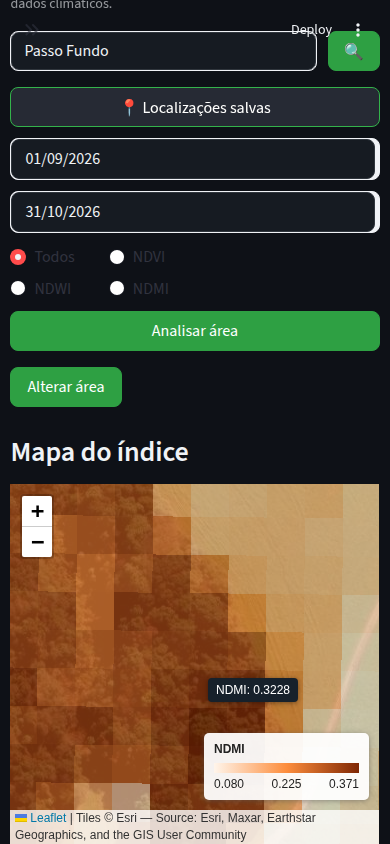
\includegraphics[width=0.74\columnwidth,height=0.43\textheight,keepaspectratio]{fig/capturas/mobile_resultados.png}
\caption{Consulta por toque e legenda NDMI em área de visualização de 390 $\times$ 844 pixels. Emulação em Chrome, não telefone físico. Fonte: captura real da aplicação local.}
\label{fig:mobile}
\end{figure}

A aplicação pode ser acessada sem instalação local pelo visitante no \href{https://eduardo198272-monitoramento-agricola-satel-streamlit-app-q0mow9.streamlit.app/}{endereço público Streamlit}. O QR Code da \cref{fig:qr-acesso} aponta para o URL completo e foi conferido por decodificação. A verificação de acesso não implica disponibilidade contínua nem publicação das correções locais.

\begin{figure}[htbp]
\centering

\includegraphics[width=0.48\columnwidth]{fig/qr_plataforma.png}
\caption{QR Code de acesso ao endereço público. Fonte: elaborado pelo autor.}
\label{fig:qr-acesso}
\end{figure}
